% !Mode:: "TeX:UTF-8"
%!TEX program  = xelatex

\documentclass[bwprint]{gmcmthesis}
\usepackage{ctex}
\usepackage{multicol}
\usepackage{bm}
\usepackage{amsmath}
\usepackage{enumerate}


\title{光传送网建模与价值评估}
\baominghao{18} %参赛队号
\schoolname{西北工业大学}%学校名称
\membera{刘恒宇} %队员A
\memberb{马旭东} %队员B
\memberc{柳俊} %队员C
\numberwithin{equation}{section}
\begin{document}
 
 %生成标题
 \maketitle
 
 %填写摘要
\begin{abstract}
本文在完成对光传送链路的编码方式,传输距离,信道特性的分析后,建立了通用的光链路传输模型,求得了在两种跨长度下三种调制格式的最大传输距离。问题一中的子问题1子问题2,通过子问题1的结果,可求出纠前误码率容限对应的三种编码方式的信噪比容限。通过分析本题给出的光传输链路的物理模型,推导信噪比与入射光功率及传输跨数的关系,得出信噪比与已传输跨数的数学关系式。由此式得出三种信噪比容限下的最大传输跨数。

然后,在问题二中,对光传输网的建模及其网络价值进行了研究,通过图论的理论将图用矩阵表达,又通过矩阵理论将网络总价值用表示了图的矩阵的运算结果表达,从而将网络规划问题转化为条件寻优问题。通过求解建立的有约束寻优模型,解析了获取光传输网络最大网络价值的网络规划方案。本文采用遗传算法计算最优的网络规划以得到最大网络价值。通过数学分析,提出计算网络价值的数学模型,确定出链路组合方式,并利用模型,求出在不同的网络价值评判标准下的最佳链路组合。但遗传算法中的种群个体数量足够多时,求得的网络规划将逼近全局最优。

最后,在问题三中,基于星座图星座点间最小间距和已调信号相位翻转两个方面,从理论分析和实际应用角度对题中给出的8QAM调制方式提出了两种改进,这两种改进均可以提高8QAM的抗噪声性能,并保持信息熵不变。






\keywords{传输建模\quad  约束寻优\quad   遗传算法\quad  信噪比}
\end{abstract}

\pagestyle{plain}

%目录 不推荐加
\tableofcontents

\newpage
%\columnseprule = 1pt
\large\centerline{\heiti 符号说明}

\begin{multicols}{2}
	$\omega_{c}$\quad 载波角频率
	
	$T_{b}$\quad N基带数字信号码元持续时间
	
	$I(t)$\quad 载波的同相分量
	
	$Q(t)$\quad 载波的正交分量
	
	$\mathrm{BER}$\quad 误比特率
	
	$\mathrm{SNR}$\quad 信噪比
	
	$n_{0}$\quad 加性高斯白噪声的功率谱密度
	
	$V_{d}$\quad 样判决门限
	
	$SNR^{thd}$\quad 信噪比容限点
	
	$S_{i}^{[m]}$\quad 光链路第m跨的输入光功率
	
	$N_{i}^{[m]}$\quad 光链路第m跨的输入噪声功率
	
	$S_{o}^{[m]}$\quad 光链路第m跨的输出光功率
	
	$N_{o}^{[m]}$\quad 光链路第m跨的输入噪声功率
	
	$SNR_{o}^{[m]}$\quad 光链路第m跨的输出信噪比
	
	$\alpha$\quad 表示光纤中的功率衰减系数
	
	$\mathrm{Gain}$\quad 光链路放大器增益
	
	$\mathrm{k}$\quad 光纤的非线性噪声功率与入纤光功率平方的比例系数
	
	$M^{*}$\quad 一条光链路的最大传输跨数
	
	$n$\quad 城市总数
	
	$\bm{p}$\quad 城市人口向量
	
	$\bm{D}$\quad 所有城市两两之间的距离
	
	$\bm{C}$\quad 所有城市两两之间连接的容量
	
	$\bm{L_{dr}}$\quad 所有城市两两之间的直接连接数
	
	$\bm{R}$\quad 所有城市两两之间的直接连接容量占该连接总容量的比率
	
	$\bm{Q}$\quad 所有城市之间两两城市人口乘积的平方根
	
	$\bm{\widetilde{C},\widetilde{L_{dr}}, \widetilde{R}, \widetilde{Q}}$分别将矩阵$\bm{C,L,R}$和$\bm{Q}$的上三角元素展开而生成的对角阵
		
	$\boldsymbol{L}_{i d r}$\quad 所有城市两两之间的间接连接数$\boldsymbol{C}_{i d r}$所有城市两两之间的间接连接容量
	

	$\boldsymbol{L}_{i d r}, \widetilde{\boldsymbol{C}}_{i d r}$\quad 分别将矩阵$\boldsymbol{L}, \boldsymbol{C}$的三角元素展开而生成的对角阵

	$\widetilde{\Lambda}$\quad 寻优算法的候选解
	
	$z$\quad $\tilde{\Lambda}$中每个对角元编码成的二进制位数 
	
	$\mathrm{s}_{k}$\quad 理想星座点
	
	$\mathrm{r}_{k}$\quad 接收到的符号
	
	$\left|s_{0}^{\max }\right|$\quad 原8QAM信号的最大幅值
	
	$\left|s_{c i r}^{\max }\right|$\quad 环形-8QAM信号的最大幅值
	
	$d_{0}^{\min }$\quad 原8QAM信号星座点间最小距离
	
	$d_{cir}^{\min }$\quad 环形-8QAM信号星座点间最小距离
	
\end{multicols}

\newpage

\section{问题重述}


\subsection{问题背景}

近年来,随着电信业的迅速发展,大量的通信新业务的不断出现,信息高速公路正在世界范围内以惊人的速度发展起来。所有这些应用都对大容量通信提出了更高的要求,光通信技术正朝着高速度、大容量、可扩展性好的方向发展。伴随着国内运营商的重组,各个运营商全业务的开展,各种业务需求的变化,对光传送网提出了新的要求。特别是近两年,光通信再次站在了技术革新的路口,以 40G/100G 、OTN 、PTN 为代表的新技术,正在将光网络向智能化、分组化和大宽带容量方向发展,一场光通信的技术革新的大幕即将拉开。

从城市内的传输,直到跨越大洋的传输,光传送网为人类提供了大容量、高可靠性和低能耗的信息传输管道,人类对通信容量的追求也成为光传送技术发展的源源不断的动力。由于人类的需求的提升,光传送网的规划与建设是运营商、设备商以及政府必须考虑的课题。光传送的基本规律是——在相同技术条件下传输的容量会随着传输距离增加而减小。网络规划者需要在有限资源的条件下,综合考虑传输距离,传输容量、网络拓扑等各种因素,以最大化网络的价值。


\subsection{需要解决的问题}

本课题中,需要站在上述角度,从底层物理出发为光传送链路建模,制定光传送网规划,探索光传送网有关规律,解决以下几个问题:

\subsubsection{问题-1:光传送链路建模}
\subsubsection*{子问题-1)纠前误码率与信噪比计算}

星座图的编码分布模式也称为调制格式,对于给定的调制格式,误码率BER和信噪比SNR呈一一对应的关系。现给出三种调制格式及编码方式,每个符号概率等概率出现,分别为QPSK,8QAM,16QAM。求出误码率BER和信噪比SNR的关系曲线,并分别计算出BER=0.02时SNR容限点的值。

\subsubsection*{子问题-2)光链路性能计算}
在单跨传输距离为80km和100km两种情况下,以纠前误码率0.02为门限,分别计算出子问题-1中的QPSK,8QAM,16QAM三种传输格式最远的传输距离(每跨距离×跨段数量)。


\subsubsection{问题-2:光传送网规划}
\subsubsection*{子问题-1)不考虑中间节点的网络规划的最优解}
12个区域,在不考虑中间节点的情况下,16条链路将区域组网。求出16条链路组合方式,使得组网网络价值最大。在16条链路的基础上,增加17条链路,求出33条链路组合方式,使得组网网络价值最大。

\subsubsection*{子问题-1)不考虑中间节点的网络规划的最优解}
当考虑存在中间节点,且两个节点可以有多个连接的情况下,重新解决子问题1),并给出所有中间节点传输容量的分配。并且考虑当区域由市扩大为省(区)时,会对结果造成什么影响。

\subsubsection*{子问题-3)考虑网络价值的评价标准,给出合适的目标函数,并得出新的网络规划。}

\newpage



\subsubsection{问题-3:改善星座图}
尝试任意改变16QAM方案中星座点的位置、数量或每个点的概率,探索8QAM(相邻各星座点之间距离相等)具有更低SNR容限点的调制方案。调制格式的信息熵需保持3bit。


\section{问题一 光传送链路建模}

\subsection{问题-1 子问题-1)解答}
基本假设:

1. M进制的各个符号之间的转换是理想的,即所有bit的转换是同时发生的,不存在中间状态。

2. 信道中的噪声是加性高斯白噪声(AWGN)。

本题图5 (a)采用非Gray码映射方式,然而,由基本假设1得,本题图5 (a)的误码率与采用Gray码映射时相同(即本题图2 (a)所示的映射方式),故而以下按照本题图2 (a)所示的映射方式分析。

\subsubsection{QPSK信号情况}
首先求出MPSK信号抗噪声性能的通解,再令M=4即为QPSK信号的情况。


\subsubsection*{MPSK信号的抗噪声性能}
多进制是利用载波的多种不同的相位状态来表征数字信息的调制方式。设载波为$cos\theta$,则M进制数字相位调制信号可以表示为

\begin{equation}
\begin{aligned}
s_{\mathrm{MPSK}}(t)&=\sum_{n} g\left(t-n T_{b}\right) \cos \left(\omega_{c} t+\varphi_{n}\right) \\ &=\cos \omega_{c} t \sum_{n} \cos \varphi_{n} g\left(t-n T_{b}\right)-\sin \omega_{c} t \sum_{n} \sin \varphi_{n} g\left(t-n T_{b}\right)
\end{aligned}
\end{equation}


式中,$g(t)$是高度为1、宽度为$T_{b}$的门函数;$T_{b}$为M进制码元的持续时间,亦即k(k =$ log_{2}M$)bit二进制码元的持续时间;$\varphi_{n}$为第n个码元对应的相位,共有M种不同取值

\begin{equation}
\begin{aligned}
\varphi_{n}=\left\{\begin{array}{l}{\theta_{1}}\quad \mbox{概率为}P_{1}\\ {\theta_{2}} \quad \mbox{概率为}P_{2}\\ {\vdots} \\ {\theta_{M}}\quad \mbox{概率为}P_{M}\end{array}\right.
\end{aligned}
\end{equation}


且
\begin{equation}
P_{1}+P_{2}+\cdots+P_{M}=1
\end{equation}
为使得平均差错概率最小,在$0\sim2\pi$之间等间隔划分相位,因此相邻相移的差值为
$$
\Delta \theta=\frac{2 \pi}{M}
$$
令
\begin{equation}
\begin{aligned}
a_{n}=\cos \varphi_{n} \\ b_{n}=\sin \varphi_{n}
\end{aligned}
\end{equation}

这样式(1)变为

\begin{equation}
\begin{aligned}
s_{\mathrm{MPSK}}(t)&=\left[\sum_{n} a_{n} g\left(t-n T_{b}\right)\right] \cos \omega_{c} t-\left[\sum_{n} b_{n} g\left(t-n T_{b}\right)\right] \sin \omega_{c} t\\
&=I(t) \cos \omega_{c} t-Q(t) \sin \omega_{c} t
\end{aligned}
\end{equation}

分别为多电平信号。所以,MPSK信号可以看成是两个正交载波进行多电平双边带调制所得两路MASK信号的叠加。MPSK信号可以用矢量图来描述,本题采用的移相方式是图1中所示的A方式。

\begin{figure}[htbp]
	\centering
	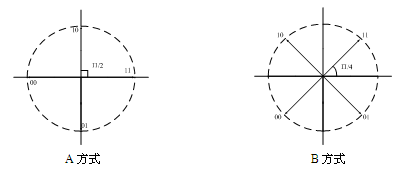
\includegraphics[width=.7\textwidth]{1.png}
	\caption{相位配置矢量图}
\end{figure}

\subsubsection*{QPSK信号的抗噪声性能}
当M=4时,MPSK信号即QPSK信号,它可以看成是由两个载波正交的2PSK信号叠加构成。其解调采用如图2所示的解调方法进行,。图中两个相互正交的相干载波分别检测出两个分量a和b,然后,经并/串变换器还原成二进制双比特串行数字信号,从而实现二进制信息恢复。
\begin{figure}[htbp]
	\centering
	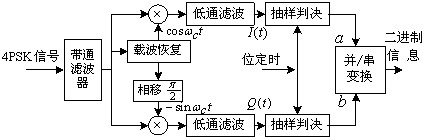
\includegraphics[width=.7\textwidth]{2.jpg}
	\caption{QPSK信号的相干解调}
\end{figure}
由于本题中BER定义为
\begin{equation}
	BER = \frac{\mbox{错误比特数}}{\mbox{总传输比特数}}
\end{equation}
所以,应该首先求出2PSK信号的抗噪声性能。
\subsubsection*{2PSK信号的抗噪声性能}

2PSK信号本质上属于DSB信号,只能采用相干解调。其相干解调系统抗噪声性能分析模型如图3所示。

\begin{figure}[htbp]
	\centering
	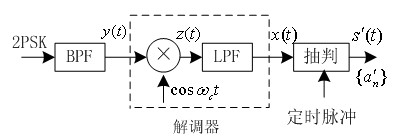
\includegraphics[width=.7\textwidth]{3.jpg}
	\caption{2PSK信号相干解调系统性能分析模型}
\end{figure}
由基本假设1得,信道噪声是加性高斯白噪声,设为$n(t)$,其均值为0,双边噪声功率谱密度为$n_{0}$/2;在一个码元持续时间(0,$T_{b}$)内,发送端发送的2PSK信号为
\begin{equation}
\begin{aligned}
S_{T}(t)=\left\{\begin{array}{c}{A \cos \omega_{c} t} \quad \mbox{发1} \\ {-A \cos \omega_{c} t}\quad \mbox{发0}\end{array}\right.
\end{aligned}
\end{equation}
则经信道传输,接收端输入信号为
\begin{equation}
y_{i}(t)=\left\{\begin{array}{c}{a \cos \omega_{c} t+n(t)} \quad \mbox{发1}\\ {-a \cos \omega_{c} t+n(t)}\quad \mbox{发0}\end{array}\right.
\end{equation}
此处,为简明起见,认为发送信号经信道传输后除有固定衰耗外,未受到畸变,信号幅度:$A\rightarrow a$。
经带通滤波器输出
\begin{equation}
\begin{aligned}
y(t)&=s(t)+n_{i}(t) \\ &=\left\{\begin{array}{c}{a \cos \omega_{c} t+n_{c}(t) \cos \omega_{c} t-n_{s}(t) \sin \omega_{c} t} \quad \mbox{发1}\\ {-a \cos \omega_{c} t+n_{c}(t) \cos \omega_{c} t-n_{s}(t) \sin \omega_{c} t}\quad \mbox{发0}\end{array}\right.
\end{aligned}
\end{equation}
其中,$n_{i}(t)=n_{c}(t) \cos \omega_{c} t-n_{s}(t) \sin \omega_{c} t$为高斯白噪声$n(t)$经BPF限带后的窄带高斯噪声,其均值为0,方差为$\sigma_{n}^{2}=n_{0} B_{2 P S K}$

取本地载波为2 $\cos \omega_{c} t$,则乘法器输出
\begin{equation}
z(t)=2 y(t) \cos \omega_{c} t\label{multiplierOutput}
\end{equation}

将式\ref{multiplierOutput}代入,并经低通滤波器滤除高频分量,在抽样判决器输入端得到
\begin{equation}
x(t)=\left\{\begin{array}{c}{a+n_{c}(t)}\quad \mbox{发1} \\ {-a+n_{c}(t)}\quad \mbox{发0}\end{array}\right.
\end{equation}
由于$n_{c}(t)$ 是加性高斯白噪声,因此,无论是发送1还是0,$x_{t}$抽样值$x$的一维概率密度$f_{1}(x)$、$f_{2}(x)$都是方差为$ \sigma_{n}^{2}$的正态分布函数,只是前者均值为$a$,后者均值为-$a$,即
\begin{equation}
f_{1}(x)=\frac{1}{\sqrt{2 \pi} \sigma_{n}} \exp \left[-\frac{(x-a)^{2}}{2 \sigma_{n}^{2}}\right]
\quad\mbox{发1}\end{equation}
\begin{equation}
f_{0}(x)=\frac{1}{\sqrt{2 \pi} \sigma_{n}} \exp \left[-\frac{(x-a)^{2}}{2 \sigma_{n}^{2}}\right]
\quad\mbox{发0}\end{equation}
令判决门限为$V_{d}$,则噪声会引起两种误码概率:

%\renewcommand{\labelenumi}{(\theenumi)}
\begin{itemize}

\item 发1错判为0的概率$P(0|1)$
\begin{equation}
\begin{aligned}
P(\mathbf{0} | \mathbf{1})&=P\left(x<V_{d}\right)=\int_{-\infty}^{V_{d}} f_{1}(x) d x=\int_{-\infty}^{V_{d}} \frac{1}{\sqrt{2 \pi} \sigma_{n}} \exp \left[-\frac{(x-a)^{2}}{2 \sigma_{n}^{2}}\right] \mathrm{d} x \\
& = \frac{1}{2}+\frac{1}{2} \operatorname{erf}\left[\frac{V_{d}-a}{\sqrt{2} \sigma_{n}}\right]
\end{aligned}
\end{equation} 

\item 发0错判为1的概率$P(1|0)$
\begin{equation}
\begin{aligned}
P(\mathbf{1} | \mathbf{0})&=P\left(x>V_{d}\right)=\int_{V_{d}}^{+\infty} f_{1}(x) d x=\int_{V_{d}}^{+\infty} \frac{1}{\sqrt{2 \pi} \sigma_{n}} \exp \left[-\frac{(x+a)^{2}}{2 \sigma_{n}^{2}}\right] \mathrm{d} x \\ &=\frac{1}{2}+\frac{1}{2} \operatorname{erf}\left[\frac{V_{d}+a}{\sqrt{2} \sigma_{n}}\right]
\end{aligned}
\end{equation} 
	
\end{itemize}

若发送1的概率为$P(1)$,发送0的概率为$P(0)$,则系统总误码率可表示为
\begin{equation}
\begin{aligned}
P_{e}&=P(\mathbf{1}) P(\mathbf{0} | \mathbf{1})+P(\mathbf{0}) P(\mathbf{1} | \mathbf{0}) \\
& = P(\mathbf{1}) \int_{-\infty}^{V_{d}} f_{1}(x) d x+P(\mathbf{0}) \int_{V_{d}}^{+\infty} f_{0}(x) d x
\end{aligned}
\end{equation}

可以看出,误码率与$P(\mathbf{1})$、$P(\mathbf{0})$、$f_{1}(x)$、$f_{0}(x)$和$V_{d}$有关。而$f_{1}(x)$和$f_{0}(x)$又与信号的抽样值$a$和噪声功率$\sigma_{n}^{2}$有关。通常$P(\mathbf{1})$和$P(\mathbf{0})$是给定的,因此误码率最终由$a$、$\sigma_{n}^{2}$和门限$V_{d}$决定。在$a$和$\sigma_{n}^{2}$一定的条件下,可以找到一个使误码率最小的判决门限电平,这个门限电平称为最佳门限电平。令
\begin{equation}
\frac{d P_{e}}{d V_{d}}=0
\end{equation}
综上,可求得最佳门限电平为
\begin{equation}
V_{d}^{*}=\frac{\sigma_{n}^{2}}{2 a} \ln \frac{P(\mathbf{0})}{P(\mathbf{1})}
\end{equation}
由题知,每个符号等概率出现,即$P(\mathbf{0})=P(\mathbf{1})=1 / 2$,此时
\begin{equation}
V_{d}^{*}=0
\end{equation}
则2PSK信号的误码率为
\begin{equation}
B E R_{2 P S K}=P_{e}=\frac{1}{2} \operatorname{erfc}\left(\frac{a}{\sqrt{2} \sigma_{n}}\right)=\frac{1}{2} \operatorname{erfc}(\sqrt{S N R})
\end{equation}

\subsubsection*{QPSK情况解答}
由于QPSK信号在进行相干解调时,输入每一个相干检测器的功率是总输入功率的1/2,即每个相干检测器的输入功率是2PSK信号情况时的一半,所以由上述分析得,QPSK信号的误码率为
\begin{equation}
B E R_{Q P S K}=B E R_{2 P S K}=\frac{1}{2} \operatorname{erfc}\left(\sqrt{\frac{S N R}{2}}\right)
\end{equation}

\begin{figure}[htbp]
	\centering
	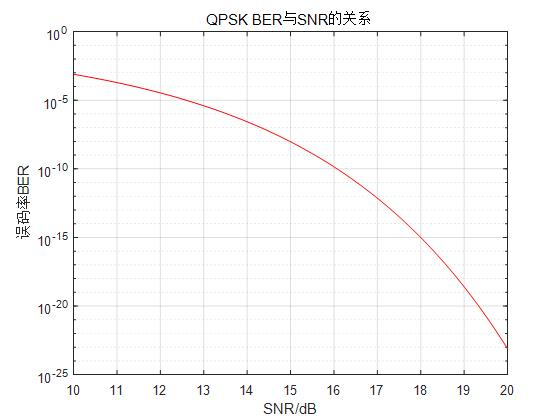
\includegraphics[width=.7\textwidth]{4.jpg}
	\caption{QPSK信号的BER与SNR的关系曲线}
\end{figure}

令$B E R_{Q P K}=0.02$时解得SNR容限点
\begin{equation}
S N R_{Q P K}^{t h d} \approx 4.2119 \approx 6.24 \mathrm{dB}
\end{equation}

\subsubsection{8QAM信号情况}

\subsubsection*{QAM信号分析}

正交幅度调制QAM源自幅度和相位联合键控APK(Amplitude Phase Keying)。APK信号是对载波的幅度和相位同时进行调制的一种方法。APK信号的一般表示式为
\begin{equation}
s_{\mathrm{APK}}(t)=\sum_{n} a_{n} g\left(t-n T_{b}\right) \cos \left(\omega_{c} t+\varphi_{n}\right)\label{apkSignal}
\end{equation}
公式\ref{apkSignal}中,$a_{n}$是基带信号第n个码元的幅度,可有L种不同的电平取值;$\varphi_{n}$是第n个信号码元的初始相位,可有N种不同的相位取值;$g(t)$是高度为1、宽度为$T_{b}$的矩形脉冲。显然,APK信号的可能状态数为L*N。将式\ref{apkSignal}展开为
\begin{equation}
\begin{aligned}
s_{\mathrm{APK}}(t)=&\left[\sum_{n} a_{n} g\left(t-n T_{b}\right) \cos \varphi_{n}\right] \cos \omega_{c} t \\ &-\left[\sum_{n} a_{n} g\left(t-n T_{b}\right) \sin \varphi_{n}\right] \sin \omega_{c} t
\end{aligned}
\end{equation}
令
\begin{equation}
\left\{\begin{array}{l}{x_{n}=a_{n} \cos \varphi_{n}} \\ {y_{n}=-a_{n} \sin \varphi_{n}}\end{array}\right.\label{apkSignal1}
\end{equation}
则式\ref{apkSignal1}可以写成
\begin{equation}
s_{\mathrm{APK}}(t)=\left[\sum_{n} x_{n} g\left(t-n T_{b}\right)\right] \cos \omega_{c} t-\left[\sum_{n} y_{n} g\left(t-n T_{b}\right)\right] \sin \omega_{c} t
\end{equation}
可见,APK信号可以看作两个正交的多进制幅度键控(MASK)信号之和,QAM信号的表达式可表示为
\begin{equation}
s_{Q A M}(t)=x(t) \cos \omega_{c} t-y(t) \sin \omega_{c} t
\end{equation}
式中
\begin{equation}
\left\{\begin{array}{l}{x(t)=\sum_{n} x_{n} g\left(t-n T_{b}\right)} \\ {y(t)=\sum_{n}^{n} y_{n} g\left(t-n T_{b}\right)}\end{array}\right.
\end{equation}
分别为同相和正交支路的基带信号,设为双极性m进制码元,$x_{n}$、y_n决定已调QAM信号在信号空间中的M个坐标点,即星座图中的M个点的位置。矩形星座图的8QAM的BER与SNR的关系如下式所示




\subsubsection*{子问题-1) QPSK情况解答}

\subsubsection{16QAM 信号情况}

\subsubsection*{MASK信号的抗噪声性能}

\subsubsection*{子问题-1) 16QAM情况解答}

\subsection{问题-1 子问题-2)}

\subsubsection{单跨传输建模}

\subsubsection{问题-1 子问题-2)求解}

\section{问题二光传送网的规划}

\subsection{模型建立}


\begin{itemize}
\item 忽略实际加工误差对设计的影响;
\item 木条与圆桌面之间的交接处缝隙较小,可忽略;
\item 钢筋强度足够大,不弯曲;
\item 假设地面平整。
\end{itemize}

\section{符号说明}

\begin{tabular}{cc}
 \hline
 \makebox[0.4\textwidth][c]{符号}	&  \makebox[0.5\textwidth][c]{意义} \\ \hline
 D	    & 木条宽度(cm) \\ \hline
 L	    & 木板长度(cm)  \\ \hline
 W	    & 木板宽度(cm)  \\ \hline
 N	    & 第n根木条  \\ \hline
 T	    & 木条根数  \\ \hline
 H	    & 桌子高度(cm)  \\ \hline
 R	    & 桌子半径(cm)  \\ \hline
 R	    & 桌子直径(cm)  \\ \hline
\end{tabular}

\section{问题分析}

\subsection{问题一分析}
题目要求建立模型描述折叠桌的动态变化图,由于在折叠时用力大小的不同,我们不能描述在某一时刻折叠桌的具体形态,但我们可以用每根木条的角度变化来描述折叠桌的动态变化。首先,我们知道折叠桌前后左右对称,我们可以运用几何知识求出四分之一木条的角度变化。最后,根据初始时刻和最终形态两种状态求出桌腿木条开槽的长度。



\subsection{问题二分析}
题目要求从折叠桌的稳固性好、加工方便、用材最少三个角度,确定设计加工参数。我们可以从应力、支撑面积考虑稳固性,从开槽长度考虑加工方便,从木板长度考虑用材最少。而它们之间又是相互制约,我们需要确定最优设计加工参数,可以建立非线性规划模型,用lingo软件来求解最优设计加工参数(平板尺寸、钢筋位置、开槽长度等),这里以合力的方向(斜向上)与最长木条(桌腿)的夹角方向最小为目标函数,以木条所承受应力小于木条的许用应力、支撑面积大于桌面面积、木条的开槽长度小于木条本身长为约束条件。
\begin{figure}[!h]
\centering
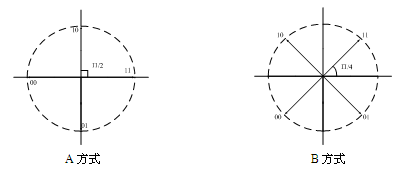
\includegraphics[width=.7\textwidth]{1.png}
\caption{问题三流程图}
\end{figure}
\subsection{问题三分析}
题目要求制作软件的意思就是客户给定折叠桌高度、桌面边缘线的形状大小和桌脚边缘线的大致形状,将这些信息输入程序就得到客户想要的桌子。我们在求解最优设计加工参数时,自行给定桌面边缘线形状(椭圆、相交圆等),桌脚边缘线形状,折叠桌高度,应用第二问的非线性规划模型,用MATLAB软件绘制折叠桌截面图,得到自己设计的创意平板折叠桌。



%参考文献   手工录入
%\begin{thebibliography}{9}%宽度9
% \bibitem{bib:one} ....
% \bibitem{bib:two} ....
%\end{thebibliography}

%采用bibtex方案
\cite{mittelbach_latex_2004,wright_latex3_2009,beeton_unicode_2008,vieth_experiences_2009}

\bibliographystyle{gmcm}
\bibliography{example}


\newpage
%附录
\appendix
%\setcounter{page}{1} %如果需要可以自行重置页码。
\section{我的 MATLAB 源程序}
\begin{lstlisting}[language=Matlab]%设置不同语言即可。
kk=2;[mdd,ndd]=size(dd);
while ~isempty(V)
[tmpd,j]=min(W(i,V));tmpj=V(j);
for k=2:ndd
[tmp1,jj]=min(dd(1,k)+W(dd(2,k),V));
tmp2=V(jj);tt(k-1,:)=[tmp1,tmp2,jj];
end
tmp=[tmpd,tmpj,j;tt];[tmp3,tmp4]=min(tmp(:,1));
if tmp3==tmpd, ss(1:2,kk)=[i;tmp(tmp4,2)];
else,tmp5=find(ss(:,tmp4)~=0);tmp6=length(tmp5);
if dd(2,tmp4)==ss(tmp6,tmp4)
ss(1:tmp6+1,kk)=[ss(tmp5,tmp4);tmp(tmp4,2)];
else, ss(1:3,kk)=[i;dd(2,tmp4);tmp(tmp4,2)];
end;end
dd=[dd,[tmp3;tmp(tmp4,2)]];V(tmp(tmp4,3))=[];
[mdd,ndd]=size(dd);kk=kk+1;
end; S=ss; D=dd(1,:);


 \end{lstlisting}


\end{document} 